\documentclass{article}
\usepackage[utf8]{inputenc}
\usepackage{graphicx}
\usepackage{caption}






\title{Relazione progetto GPU computing}
\author{Martino Tiziani}
\date{Maggio 2019}

\begin{document}

\maketitle

\section{Attacco Algebrico}

Un'attacco algebrico è un particolare tipo di attacco crittografico che fa uso dell'algebra lineare per attaccare un cifrario. La tecnica si compone di due fasi:

\begin{itemize}
\item \textbf{fase di traduzione}: si effettua una traduzione del cifrario, che deve essere attaccato, in un sistema di equazioni polinomiali con coefficienti in un campo finito (il modulo è quindi un numero primo).

\item \textbf{fase di risoluzione}: in questa fase si risolve il sistema di equazioni appena trovato e dalla soluzione è possibile estrarre la chiave segreta del cifrario originale (o parte di essa).

\end{itemize}

Questo attacco è molto interessante per via della sua versatilità, infatti questa tecnica è applicabile a tutti i cifrari che sono scrivibili come un sistema di equazioni, la grande potenzialità è che tutti i cifrari realizzati fino ad oggi possiedono questa caratteristica. 

L'attacco algebrico risulta quindi un attacco che può essere utilizzato su qualsiasi cifrario, tuttavia è ancora poco conosciuto, rispetto ad altre tecniche di crittoanalisi, questo è dovuto alla sua complessità computazionale. Infatti senza entrare troppo nel dettaglio nella teoria della complessità la fase di risoluzione di un sistema di equazioni lineari in campo finito è classificato come NP-complete. Un problema con questa complessità risulta irrisolvibile, in un tempo accettabile, per istanze di grosse dimensioni, e anche con piccole dimensioni i tempi di esecuzione sono elevati. Tuttavia il parallelismo potrebbe portare in alcuni casi dei benefici da non sottovalutare.

\section{Risolvere il sistema}

Risolvere il sistema di equazioni che descrive il cifrario in discusisone è il punto centrale dell'attacco algebrico. Esistono diverse tecniche per risolvere tale sistema, alcune banali altre più ricercate e complesse. Molte di queste tecniche hanno benefici su particolari istanze di problema o in determinate condizioni. Il sistema di risoluzione qui esposto (realizzato come lavoro di tesi) si compone di due fasi: 

\begin{itemize}
\item \textbf{fase di espansione}: si espande il sistema aggiungendo delle equazioni in modo tale che il sistema risulti risolvibile.
\item \textbf{fase di riduazione}: si riduce il sistema con l'algoritmo di riduzione di Gauss (si eliminano le equazioni linearmente dipendenti).

\end{itemize}

Si ripetono queste fasi fino alla soluzione completa del sistema. La fase di espansione è necessaria perché il sistema di partenza non è, quasi mai, direttamente risolvibile, ovvero non possiede sufficienti equazioni.

\section{Riduzione di Gauss e parallelismo}

Il Fulcro di tutto il sistema realizzato è la riduzione di Gauss di un sistema di equazioni modulari. Questo algoritmo rappresenta il sistema sotto forma di una matrice e ripete su di essa un set di operazioni consentite.
\begin{itemize}
\item scambiare due righe
\item moltiplicare una riga per un numero diverso da zero
\item sommare alla riga il multiplo di un'altra riga
\end{itemize}

Lo scopo dell'algoritmo è trasformare la matrice di partenza in una matrice a scalini. Ottenuta questa forma il sistema può essere facilmente risolto per sostituzione inversa. Fortunatamente questo algoritmo è per sua natura parzialmente parallelizzabile. Ci sono diverse varianti di questo algoritmo, qui viene utilizzata la riduzione di Gauss con pivot completo. Come da pseudocodice si nota che i due cicli interni effettuano operazioni completamente indipendenti su dati indipendenti, percio tali operazioni possono essere eseguite completamente in parallelo. Nella realizzazione del sistema si è sfruttato il parallelismo su CPU per velocizzare il più possibile la computazione, tuttavia data la natura fortemente parallela di una porzione dell'algoritmo è senza dubbio interessante verificare come il parallelismo di una GPU possa influenzare tale computazione.

\section{Implementazione CUDA}

Come detto in precedenza esistono tanti metodi per risolvere il sistema in esame, la riduzione di gauss è senza dubbio uno dei metodi più banali, tuttavia fornisce al programma una generalità (non sfrutta nessuna condizione specifica, funziona sempre) che le altre tecniche non forniscono. La stessa riduzione di Gauss può essere effettuata in diversi modi, ciononostante lo scopo di questo progetto è quello di comparare l'implementazione parallela realizzata su CPU con quella per GPU, per cui non vengono utilizzate diverse risoluzioni come ad esempio la decomposizione LU, o altre.

Il problema e gli elementi su cui bisogna lavorare sono espressi più chiaramente dalla Figura \ref{fig:mat}. Si noti che, dopo aver identificato una colonna e riga pivot (celle arancione), deve essere ridotta tutta la sottomatrice (di colore giallo) sottostante il pivot per ottenere l'i-esimo scalino (colonna pivot ridotta a 0 a partire dalla riga sottostante il pivot). La riduzione di questa porzione di matrice può avvenire in modo completamente parallelo.

	\begin{center}
		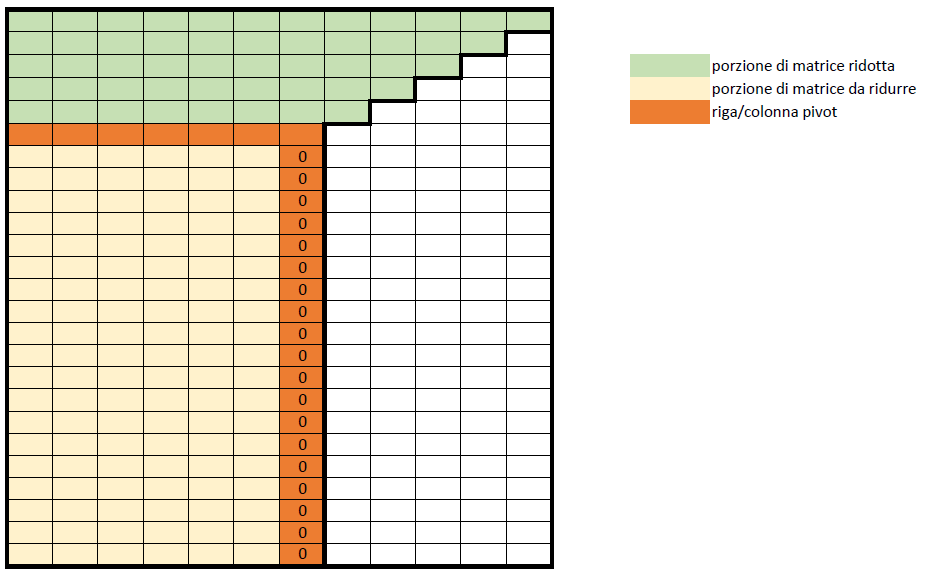
\includegraphics[width = \textwidth]{matrice.png}
		\captionof{figure}{Schema della struttura della matrice}
		\label{fig:mat}
	\end{center}


Sono state realizzate tre tecniche per ridurre la porzione di matrice gialla:
\begin{itemize}
\item \textbf{celle}: il kernel effettua la riduzione di una sola cella
\item \textbf{righe}: il kernel effettua la riduzione di una riga 
\item \textbf{blocco}: il kernel effettua la riduzione di un blocco della colonna
\end{itemize}


Prima di procedere oltre è necessario riflettere su come implementare il ciclo esterno, tale operazione infatti non è parallelizzabile. Si possono adottare due scelte:
\begin{itemize}
\item effettuare il ciclo esterno su CPU in modo veloce ed efficiente per poi trasferire su GPU la matrice e risolvere la riduzione in parallelo.
\item effettuare il ciclo esterno su un singolo kernel in modo poco efficiente e sfruttare il \textbf{parallelismo dinamico} per lanciare la riduzione successiva.
\end{itemize}

La prima tecnica per quanto possa sembrare appetibile non è utilizzabile, in quanto il numero di trasferimenti della matrice risulta essere troppo elevato, quando la dimensione della matrice inizia a crescere i trasferimenti diventano insostenibili. La seconda tecnica sacrifica le performance del ciclo esterno per mantenere la matrice sempre in memoria globale della GPU evitando continui e costosissimi trasferimenti di memoria con la CPU. Per tanto si sono realizzate le tre tecniche precedenti sfruttando il parallelismo dinamico.

\section{Risultati ottenuti}

Di seguito si forniscono i risultati ottenuti con le tre diverse teniche: cella, riga, blocco. Non si espone ne si commenta esplicitamente il codice realizzato per brevità e chiarezza. 



\end{document}